\documentclass[a4]{article}
\usepackage{gnuplottex}
\usepackage{csvsimple}
\usepackage{subcaption}
\usepackage{amsmath}
\usepackage{graphicx}
\usepackage{epstopdf}
\usepackage{float}

\graphicspath{ {./image/} }

\title{COMP26120 Lab 3 Report}
\author{Ziyi Li}
\begin{document}
\maketitle

\section{Experiment 1}

In this experiment, I use mode 4 in my program. The hash value of a string is calculated by:
$$ h(s) = (a * sum + b) \  mod \  s.length$$
where s is a string, and a,b,sum are calculated by:
$$ a(s) = ord(s[0])^2$$
$$ b(s) = ord(s[-1])^3$$
$$ sum(s) = \sum^{s.length}_{i=0}(ord(s[i])^3)$$


\subsection{Hypothesis}

Any distinct string would get a unique hash value that represents its coordinate in the array. 
So the complexity of both insert and search is O(1)
\\ \hspace*{\fill} \\
\noindent This is the ideal situation, when the size of HashSet is enough, every element will have a unique hash value. When inserting the data, it can always find a free place(unoccupied) place and store it. It is the same with search, the program calculates the hash value of the data and finds the data in the place of that value directly. However, in real situations, it is possible that collisions happen, which means the place of that value should be has been occupied. So we need to apply the store procedure with collision, which is to search after that index linearly until finding a free place. When the pointer reached the end of the array, jump back to the start. 
I already applied occupation rate detection of the whole set, when the rate is larger than 0.5, resize will be applied, so it is not possible that the array is full.

\subsection{Design}

Python Jupyter notebook is used to test the hypothesis. The test file is in python hashset\_report.ipynb

\noindent Initial size of HashSet is (length of test file / 0.5).

\noindent The test data is a list containing N random strings (word length is 10).

\noindent Tests will insert all words and then search all words. The hit rate is 100\% which means there will be no failure when searching.

\noindent The size of the test set starts from 100 and ends with 100000, the step is 100.



\subsection{Results}

The result is in file hashset\_mode4\_result.csv

Definition:

Avg insert - The average step of finding address to insert element

Avg find - The average step of finding address and compare with element

Collision rate - Total collision number divides hashset size
\\

\begin{figure}[H]
    \begin{minipage}{0.48\textwidth}
    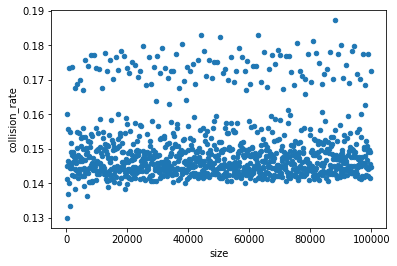
\includegraphics[width=0.95\textwidth]{h-size-collision.png}
    \caption{Size - Collision rate}
    \end{minipage}
    \begin{minipage}{0.48\textwidth}
    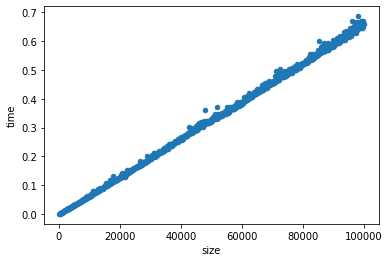
\includegraphics[width=0.95\textwidth]{h-size-time.png}
    \caption{Size - Time}
    \end{minipage}
    \begin{minipage}{0.48\textwidth}
    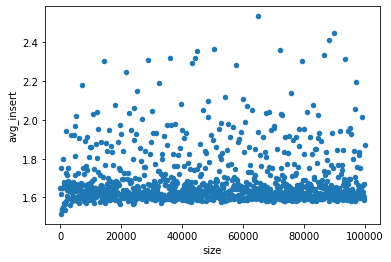
\includegraphics[width=0.95\textwidth]{h-size-insert.png}
    \caption{Size - Avg insert}
    \end{minipage}
    \begin{minipage}{0.48\textwidth}
    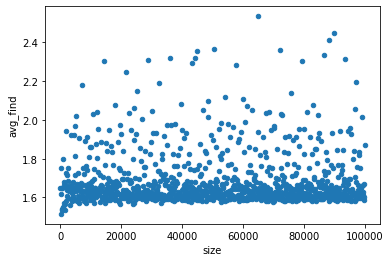
\includegraphics[width=0.95\textwidth]{h-size-find.png}
    \caption{Size - Avg find}
    \end{minipage}
\end{figure}

\subsection{Discussion}

Program runtime grows with the size of the data set and is almost proportional. This is logical because as the number of data increases, the time to complete all inserts and lookups increases in equal proportion.\\

\noindent To compare the complexity of program runs, we focus on the average number of operations, these values represent the running time of the program for each read or write operation. The values of avg insert and avg distributed in a certain interval, there is no change in the range with data size. This trend is also seen in the collision rate, the percentage does not change with size. The operation cycle did not raize with the size of the data which means both insert and find operation can completed in a small number of cycles. This fits the O(1) although not perfectly.\\

\noindent However the query hit rate in my test file is 100\%, which means everything that the program searched is in HashSet, there was no situation in the value was not fount in HashSet. This is a reason why operation cycles did not increase.\\

\noindent I optimize for the "element not found" case so that the worst-case complexity is less than O(n). When the hash position of an element is empty, or the hash position is occupied but the next position is empty (and so on), we can just return the element not found because it is not in the position it should be. Most of the time we don't need to look for it in a complete linear fashion, so this will be much more efficient. Of course, the current programming does not take into account deleting elements.

\subsection{Conclusion}

The hypothesis that the time complexity of hashset algorithm is O(1) is satisfiable.

\section{Experiment 2}

In this experiment, the binary search tree will be used.

\subsection{Hypothesis}

The time complexity of binary search tree algorithm is O(h) where h is the height of the tree.

This means when the height increase, the time complexity will proportionally increase.

\subsection{Design}

Python Jupyter notebook is used to test the hypothesis. The test file is in python bstree\_report.ipynb

\noindent The test data is a list containing N random strings (word length is 10).

\noindent Tests will insert all words and then search all words. The hit rate is 100\% which means there will be no failure when searching.

\noindent The size of the test set starts from 100 and ends with 100000, the step is 100.

\noindent Here we count the relationship between the height and the number of operations. Average operation numbers are calculated with total access time divided size of data.


\subsection{Results}

The result is in file bstree\_result\_result.csv

Definition:

Avg insert - The average comparison steps to insert element

Avg find - The average comparison steps to finding the element

\begin{figure}[H]
    \begin{minipage}{0.48\textwidth}
    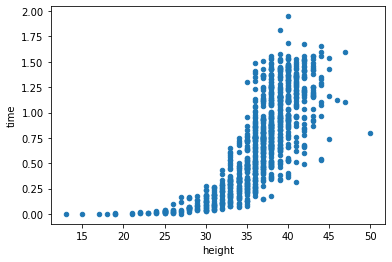
\includegraphics[width=0.95\textwidth]{b-height-time.png}
    \caption{Height - Time}
    \end{minipage}
    \begin{minipage}{0.48\textwidth}
    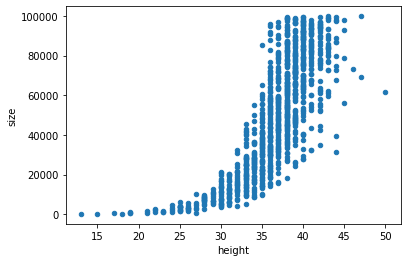
\includegraphics[width=0.95\textwidth]{b-height-size.png}
    \caption{Size - Height}
    \end{minipage}
    \begin{minipage}{0.48\textwidth}
    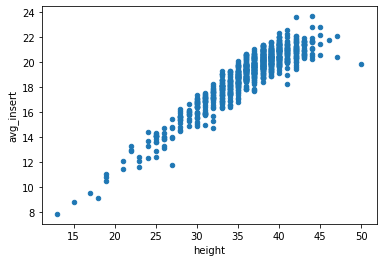
\includegraphics[width=0.95\textwidth]{b-height-insert.png}
    \caption{Size - Avg insert}
    \end{minipage}
    \begin{minipage}{0.48\textwidth}
    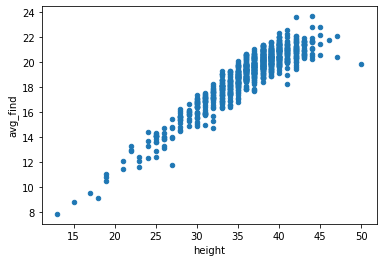
\includegraphics[width=0.95\textwidth]{b-height-find.png}
    \caption{Size - Avg find}
    \end{minipage}
\end{figure}

\subsection{Discussion}

As the size of the dataset increases, the height of the binary search tree increases as well. The effect of the increased height is an increase in program runtime, as more comparisons are required for each lookup. This increasing trend is exponential. Since there is no direct relationship between dataset size and height, there are cases where there are different dataset sizes but the same height, so there are multiple points on the chart distributed on the same height axis.\\

\noindent To study the complexity of this algorithm, we mainly compare the relationship between the number of operations and the height, just as defined. In this experiment I didn't consider the worst case, the test data set is set to every element that can be found in binary search tree. As the result from the charts, we can see that the average operation cycles rise with the height of the binary search tree, and this growth trend fits the line of positive proportion.

\noindent In worst cases, we can imagine that the complexity of each operation is h, this will also be a positive proportional growth curve, but the program will take much longer to run.
\subsection{Conclusion}
The hypothesis that the time complexity of binary search tree is O(h) is satisfiable.\\

\section{Appendix}

%% And raw data or code scripts you want to present should be included as appendices.
The data is too long to be inserted into this document. The files mentioned below are stored in the lab3/python folder

\begin{itemize}
\item hashset\_report.ipynb - The program is used to automatically run insert and find with mode 4 of HashSet, then statistic the data of each cycle and generate raw data and charts.
\item hashset\_mode4\_result.csv - The raw data generated by program hashset\_report.ipynb.
\item bstree\_report.ipynb - The program is used to automatically run insert and find with binary search tree, then statistic the data of each cycle and generate raw data and charts.
\item bstree\_result.csv - The raw data generated by program bstree\_report.ipynb.
\end{itemize}


\end{document}